\chapter{Expert priors in compartmental models: bipolar disorder}
\label{applications-prior_level_vals}

Just as priors in the spline model were influential on the estimates
produced for PMS prevalence in
chapter~\ref{applications-priors_knots_select}, the priors on the
age-specific rates in a compartmental model can be influential on the
estimates.  The situation is more complicated here, however, because
priors on a hazard of one type propagate through to affect the
estimates for all other parameters as well, due to the consistency
enforced by the compartmental model.  In this chapter, we will use the
meta-analysis of bipolar disorder prevalence as an example of the
effects of informative priors on levels of age-specific incidence and
remission hazards.

Bipolar disorder is a mental disorder that causes the experience
of at least one manic and one major depressive episode,
interspersed by periods of residual symptoms.  A manic episode is
characterized by elevated, expansive, or irritable mood, while a
depressive episode is characterized by depressed mood or loss of
interest in everyday activities.  A shift between episodes is
demarcated by either a change in symptoms to the opposite polarity
or experiences of residual symptoms that are below the threshold
for a manic or depressive episode.  In the case of rapid cycling,
shifts between episodes occur as frequently as four or more shifts
in a given year.  Extreme behavior
changes accompany mood changes, and it is not uncommon for sleeping,
eating, or activity patterns to change with manic and depressive
episodes.
While there
is no cure, treatment helps manage mood swings and related
symptoms. \cite{kloos_bipolar_2011, angst_historical_2000, TK_coauthor_ref}

The modeling of bipolar disorder is based on literature describing it
as a chronic illness with little or no complete remission.
The terms ``residual'' and ``remission'' have very different implications
for the GBD 2010 Study.  A residual state involves less severe
symptoms with lesser disability but still contributes to disease
burden.  Remission is equivalent to a cure rather than a temporary
reduction in symptom levels and thus does not contribute to burden.  No studies
were found reporting on complete remission from bipolar disorder as per this definition,
which is consistent with the description in the literature that there
is no cure. \cite{american_psychiatric_association_diagnostic_2000}
In this chapter, analysis
uses only data from the GBD 2010 Study region of North America, High Income,
shown in figure~\ref{fig:app-bipolar data}.

    \begin{figure}[h]
        \begin{center}
            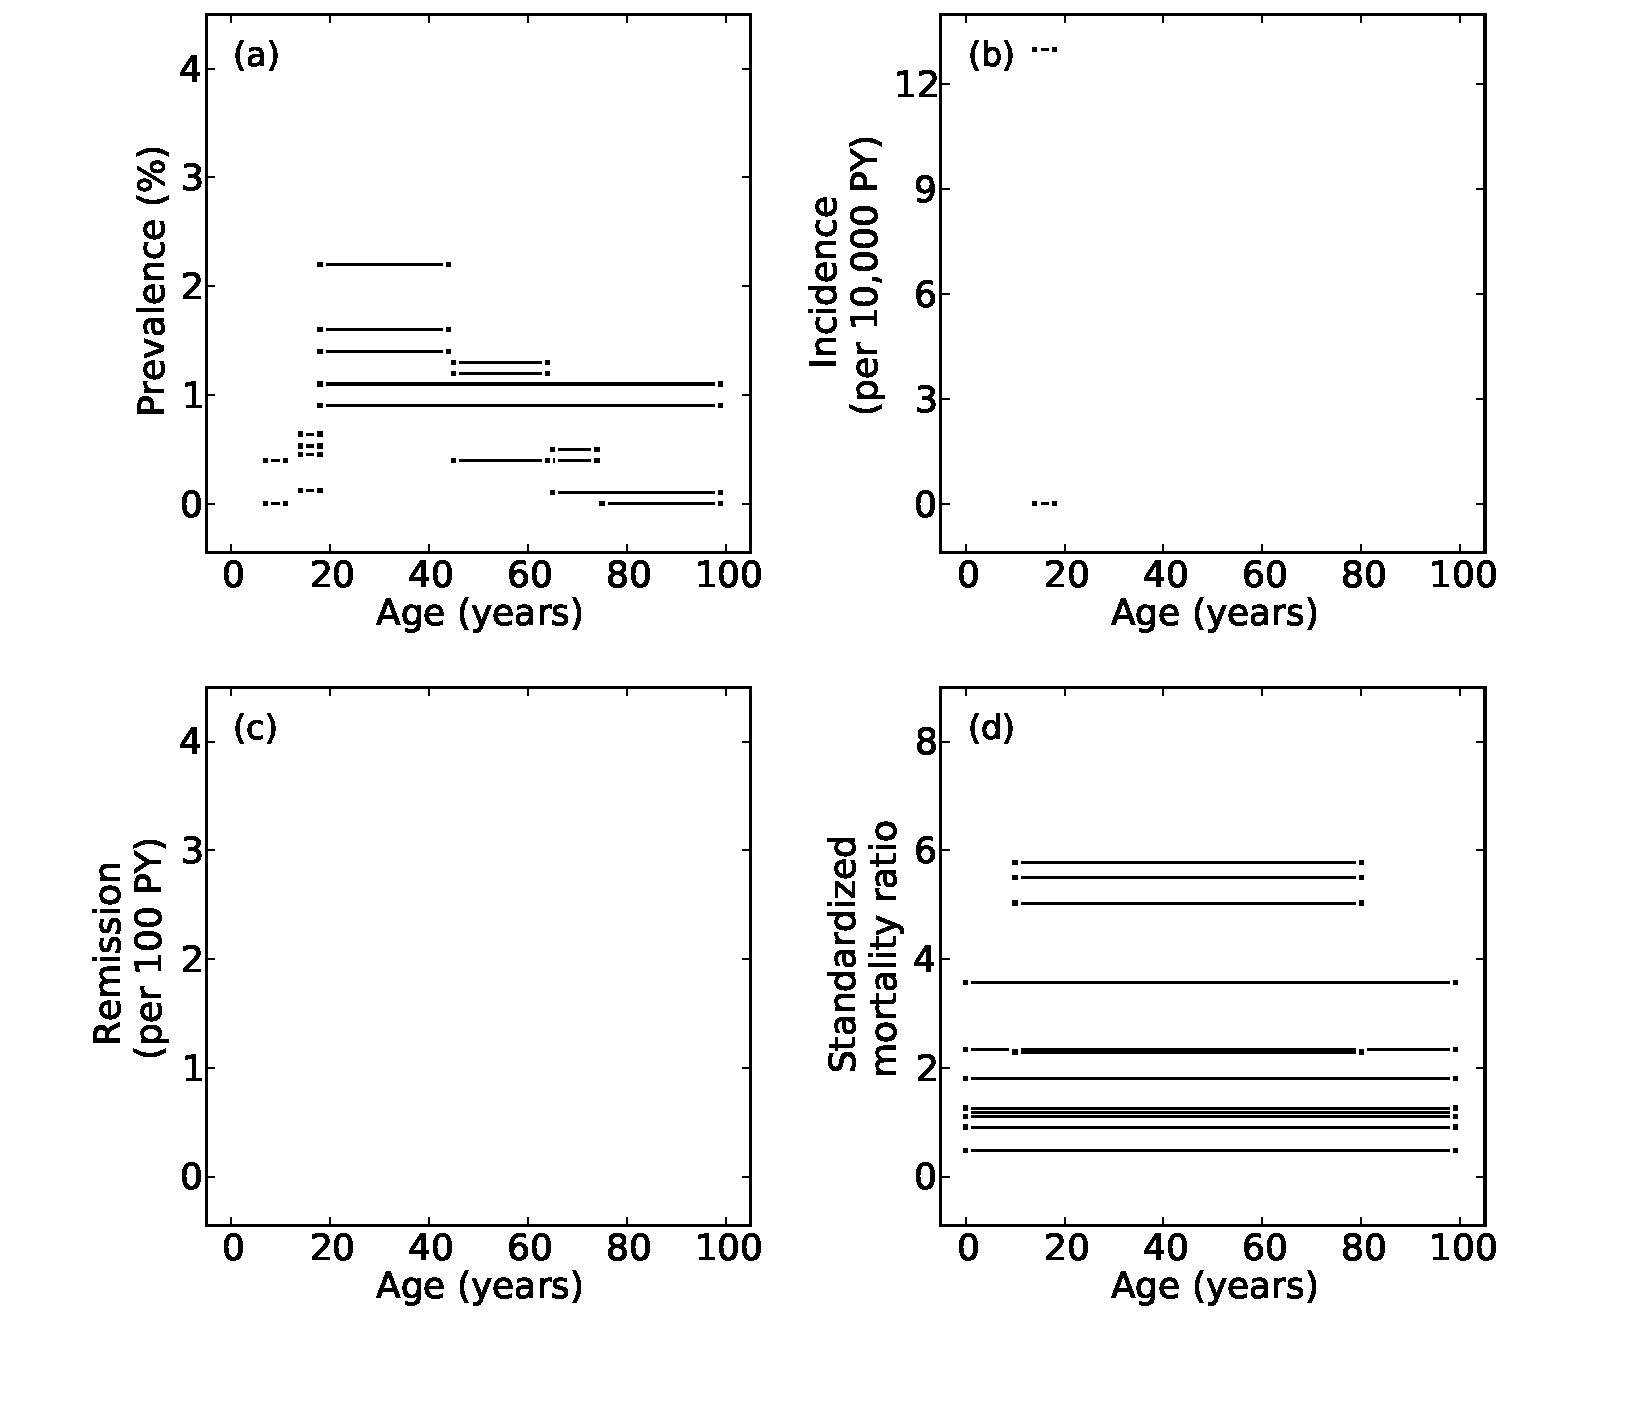
\includegraphics[width=\textwidth]{bipolar-data.pdf}
            \caption[Systematic review data for bipolar disorder.]{Data on 
            (a) prevalence, (b) incidence, (c) remission, and
              (d) standardized mortality ratio collected from systematic review
              of bipolar disorder in the GBD 2010 Study
              region of North America, High Income.}
            \label{fig:app-bipolar data}
        \end{center}
    \end{figure}

%\section{Prevalence and Incidence age of onset}
While there is evidence to suggest that bipolar disorder commonly
starts in the midteens or early twenties, there is still disagreement
over a minimum age of onset.  Even though symptoms can be tracked back
to childhood, setting a threshold for diagnosis is difficult given
that current diagnostic criteria are based on the adult presentation of
the disorder.  Literature and expert advice suggest that although
prepubertal bipolar disorder is rare, there is a possibility it may
exist. \cite{kloos_bipolar_2011, angst_historical_2000}

While expert priors are useful in guiding the modeling process, they
may have unintended effects, as discussed in chapter~\ref{theory-expert_priors}.
Choosing to have no restrictions on the
age of onset alters the age-specific prevalence greatly, as shown in
figure~\ref{fig:app-bipolar bounds}.

    \begin{figure}[h]
        \begin{center}
            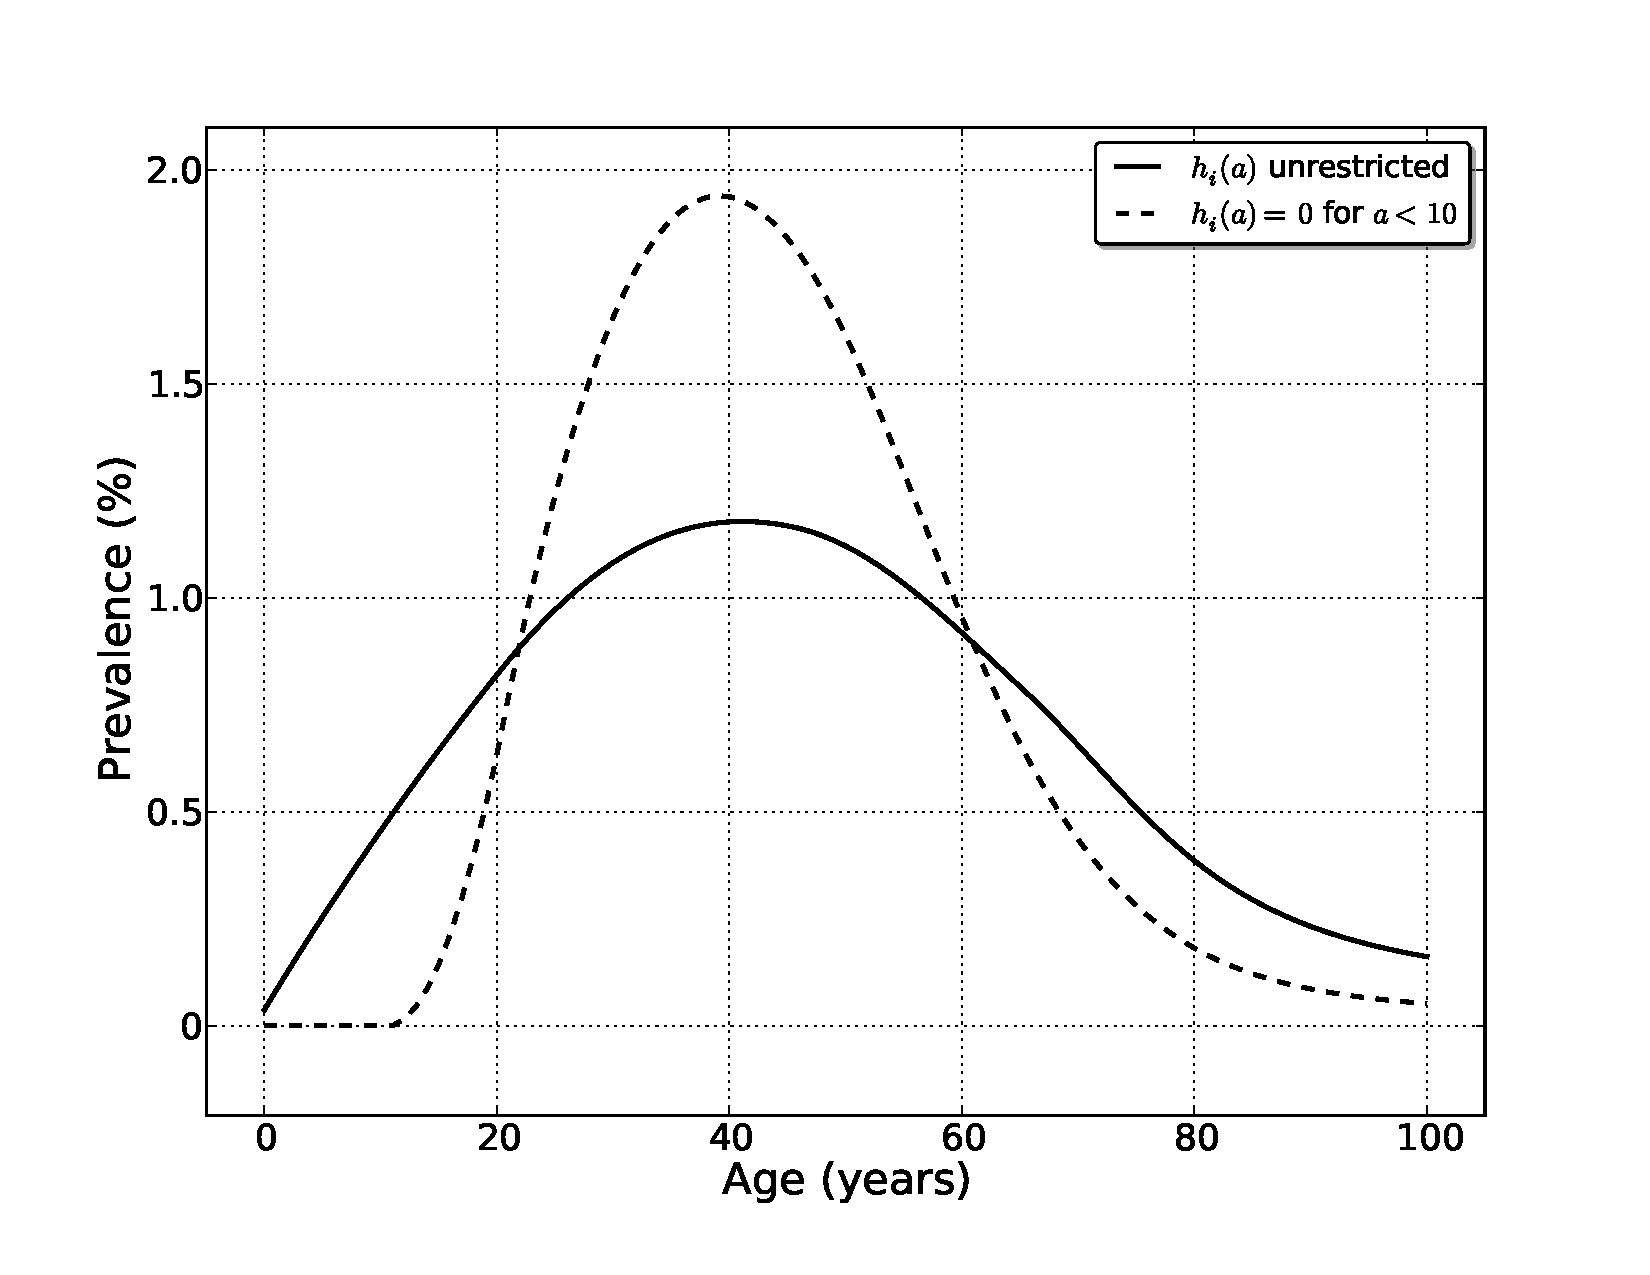
\includegraphics[width=\textwidth]{bipolar-bounds.pdf}
            \caption[Comparison of prevalence estimates for bipolar disorder
              using differing priors for the age of onset in a compartmental
              modle.]{Estimates of the prevalence of bipolar disorder
              for males in the GBD 2010 Study region of North America, High Income,
              in 1990 using differing priors for age of onset
              in a compartmental model.}
            \label{fig:app-bipolar bounds}
        \end{center}
    \end{figure}

Like the age of onset, little is known about the upper age limit of
bipolar disorder.  Using expert knowledge to set plausible bounds on the
level of disease is useful in modeling noisy data.  However, changes in the upper age
limit may produce unexpected changes, as shown in figure~\ref{fig:app-bipolar onset}.
The prevalence estimates in figure~\ref{fig:app-bipolar onset} are about
the same because there are enough data to inform the model, but incidence,
remission, and excess mortality undergo subtle changes to account for the prior.

    \begin{figure}[h]
        \begin{center}
            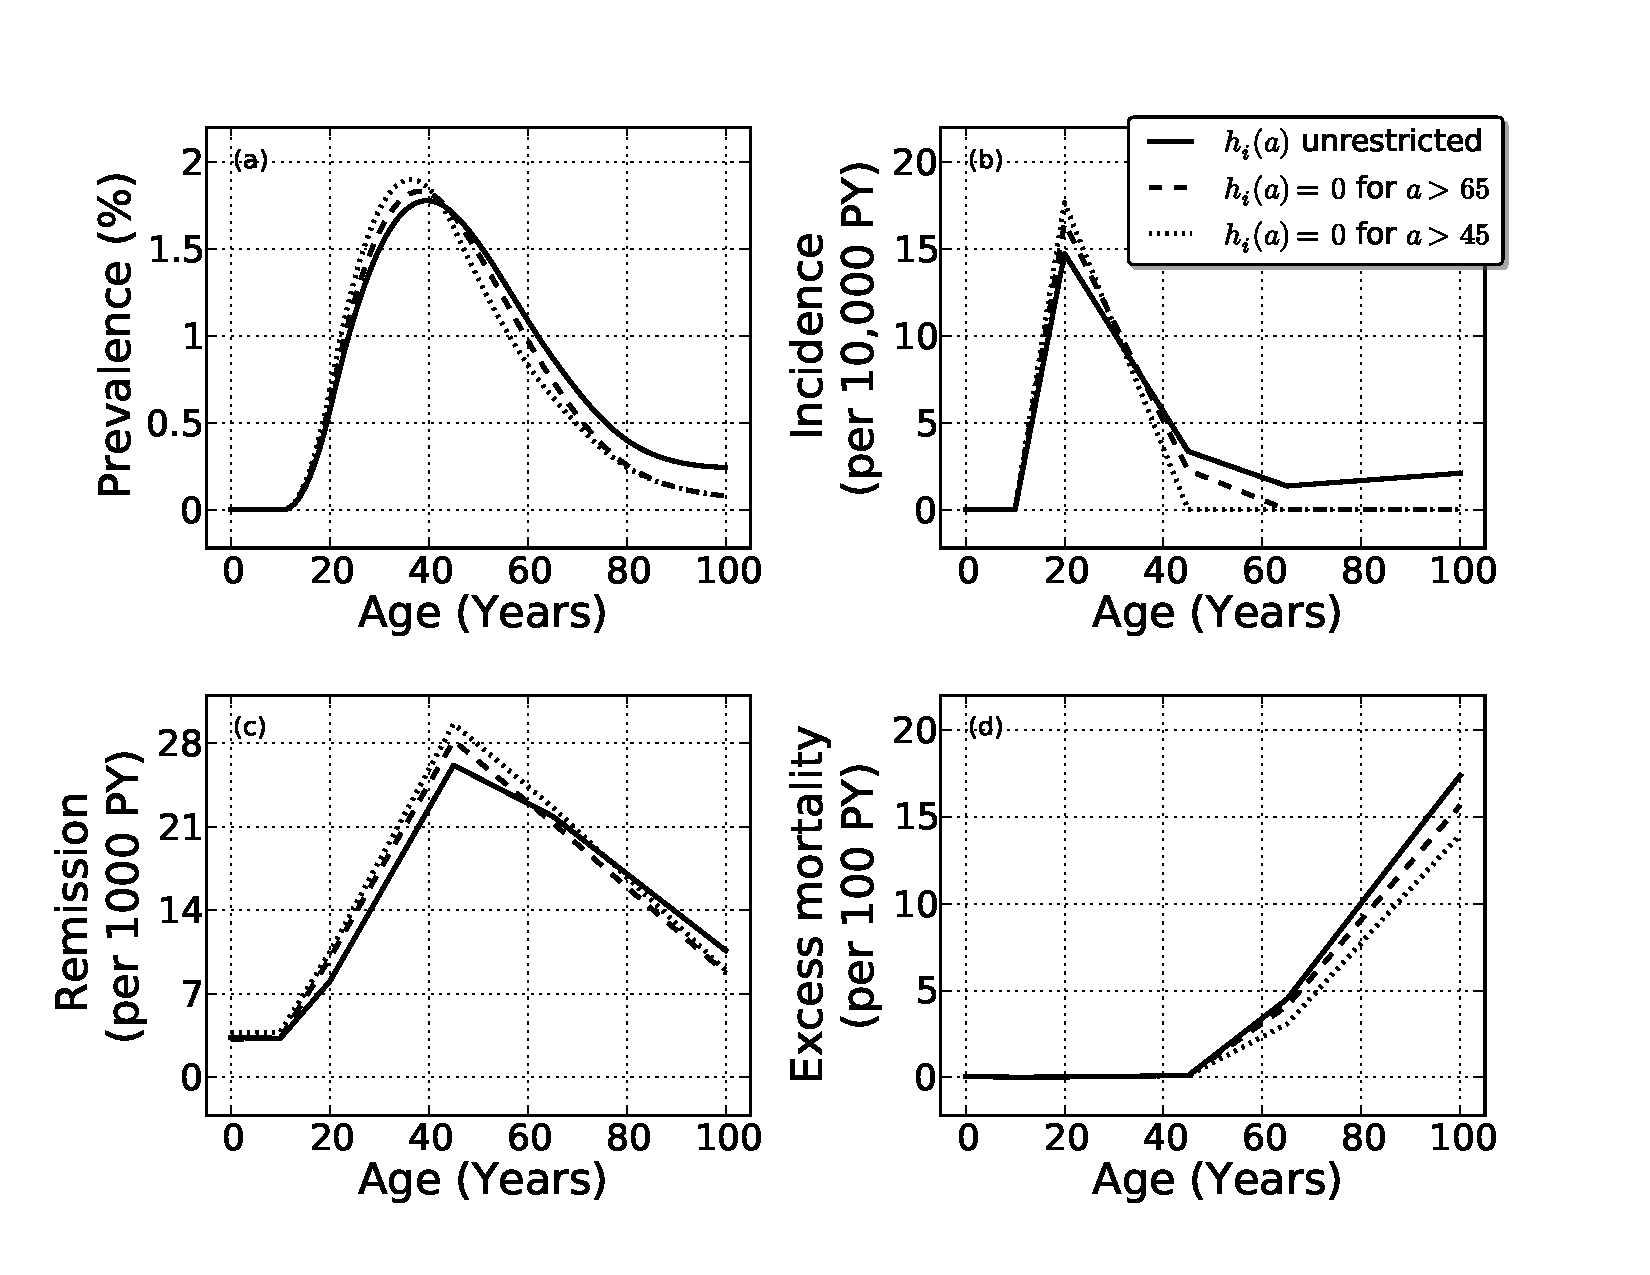
\includegraphics[width=\textwidth]{bipolar-45_65_100.pdf}
            \caption[Comparison of estimates for bipolar disorder using 
              a compartmental model with different priors on the upper
              age limit of incidence.]{Estimated (a) prevalence, (b) 
              incidence, (c) remission, and
              (d) excess mortality for males with bipolar
              disorder in the GBD 2010 Study region of North America, High Income,
              in 1990 using a compartmental model with
              different priors on the upper age limit of
              incidence of $45$ years, $65$ years, or unrestricted.}
            \label{fig:app-bipolar onset}
        \end{center}
    \end{figure}

%\section{Residual v Remission}
In sparse and noisy data, sometimes the changes to account for the prior
are not so subtle, as shown in the sensitivity analysis in
figure~\ref{fig:app-bipolar remission}.  Here, small changes in the
prior level on remission lead to large changes in the estimated excess mortality.

    \begin{figure}[h]
        \begin{center}
            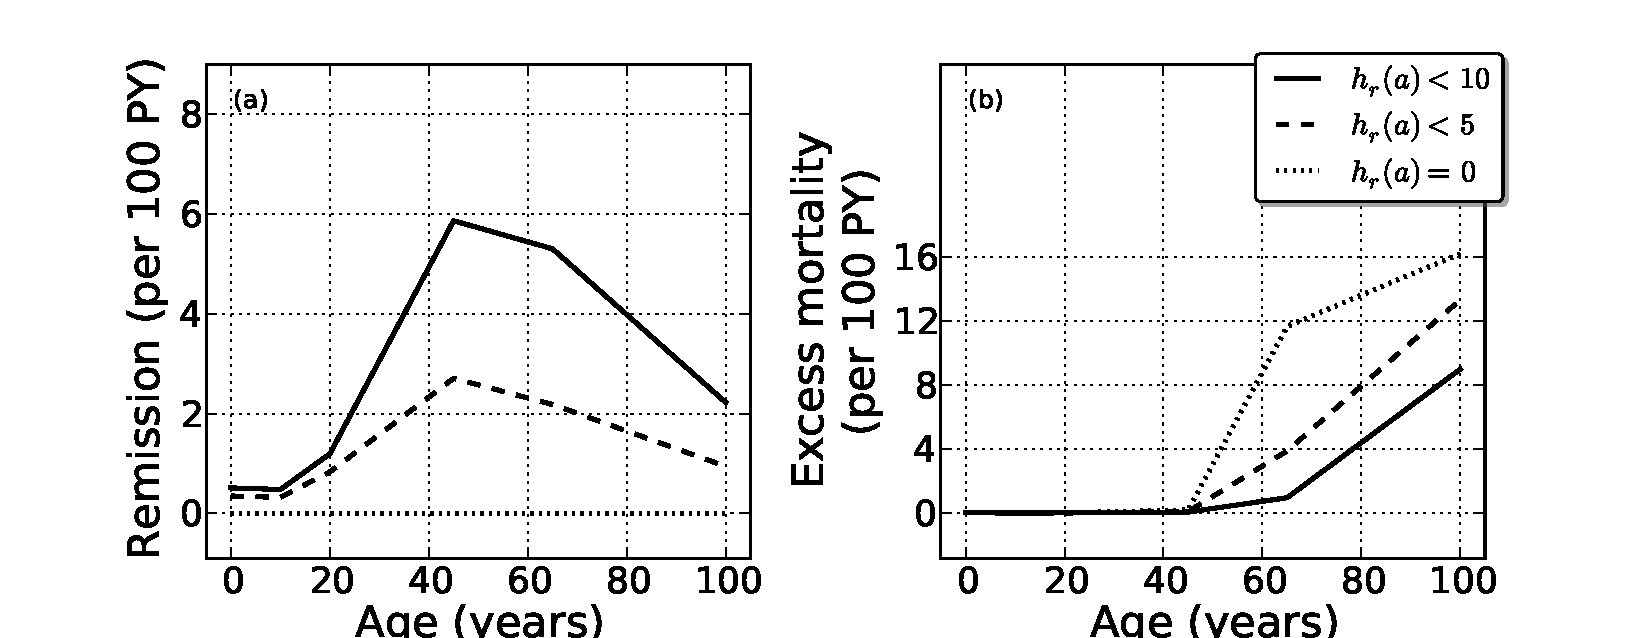
\includegraphics[width=\textwidth]{bipolar-0_5_10.pdf}
            \caption[Comparison of estimates for bipolar disorder using a 
              compartmental model with different priors on remission.]{Estimated 
              (a) remission and (b) excess
              mortality for bipolar disorder in
              males in the GBD 2010 Study region of North America, High Income,
              in 1990 in a compartmental model
              with different priors on remission that limit remission
              to 0, 5, or 10 per 100 PY.}
            \label{fig:app-bipolar remission}
        \end{center}
    \end{figure}

The internal consistency in the compartmental model causes modeling
decisions, such as priors on level, for one parameter to propagate and
affect all other parameter estimates.  When working with ample data,
the model estimates are robust against the choice of informative priors on
level.  However, these choices can cause substantial changes to
estimates when working with sparse and noisy data.




